\documentclass{ctexart}

\title{基于通用协议的五子棋引擎设计与实现}
\author{胡玮文}
\date{2019/1/1}

\usepackage{hyperref}
\usepackage{amsmath}
\usepackage[margin=3cm]{geometry}

\begin{document}

\maketitle
\newpage

\paragraph{摘要} 本文介绍了一个基于通用协议的五子棋引擎的设计与实现。使用C\#编程语言,基于.NET Framework和.NET Core平台实现,采用高度模块化的构造,实现了通用协议\cite{WEBSITE:protocol}的通信方法,实现了Alpha Beta剪枝算法,及杀手启发等来自网络上或是我独立发明的优化方法。另外,作为棋力的对照,我复用了大多数模块实现了一个基于蒙特卡洛树搜索算法的五子棋引擎。作为成果,本引擎可以在piskvork\cite{WEBSITE:piskvorky}程序中与人类棋手或者其他引擎对战。我也实现了一个简易的AI对战平台,用于评测我的引擎的不同参数对棋力的影响;同时也实现了一个性能测试平台,用于评测代码的不同部分对性能的影响,并依此改善程序的性能。本工作的亮点在于,引擎的棋力较高,在有一百余人的班级中举行的AI比赛中,本引擎毫无悬念地取得了冠军。本引擎在实现上没有使用现有的任何关于五子棋的代码,的每一个组件均为从头开始实现的。

\paragraph{关键字} Alpha Beta剪枝;杀手启发;五子棋AI;零和博弈;五子棋通用协议

\section{介绍}
随着Deep Mind公司的Alpha Go与Alpha Zero\cite{ARTICLE:AlphaZero}在围棋等完全信息零和博弈问题中的出色表现,使得大家对这方面的研究又充满了兴趣。特别是Alpha Go Zero只使用强化学习方法在自我对弈中学习,在围棋游戏上达到了超越世界冠军的水平。这让人们对计算机的学习能力有了新的期待,同时也体现出了算法的强大力量。在大三上学期的人工智能课程上,我们学习了博弈树,搜索,以及Alpha Beta剪枝算法的相关概念,并且在课程实验任务中实现了本文介绍的引擎。本引擎在设计时也希望能最小化人类知识在引擎中的作用,在实现时优化的目标也集中于如何通过改进算法来提高棋力,而不是如何更好地将人类的已有知识编码进程序里。以此凸显算法的力量。

\section{算法}

\paragraph{Alpha Beta剪枝} 本引擎中实现的Alpha Beta剪枝算法是负极大值形式的,这样实现的时候代码更加简洁,分支更少。其核心思想和传统的Alpha Beta剪枝算法是一致的,即只需要搜索到一个足够好(坏)的结果即可,而不需要知道它究竟有多好(坏)。在递归搜索时每次递归都给出一个Alpha和Beta值作为分数的上界和下界,在搜索过程中只需要分数超出了这个范围便可提前返回(剪枝)。

这是一个保守的剪枝算法,使用这种剪枝后依然可以保证自己在已搜索完的层数内不会被杀(除非已经必败了),也不会错过任何在已搜索完的层数内杀死对手的机会。

该算法剪枝的表现大大依赖于走法排序的措施,对当前走子方有利的走法排在前面时,剪枝效果更佳,实际搜索的分支因子就更小。而这也是后面将要介绍的很多优化算法的用武之地。

\paragraph{迭代加深} 由于Alpha Beta剪枝是建立在深度优先搜索的基础上的,而博弈树的深度可能非常深,所以我们必需限制搜索的深度。迭代加深算法的思想就是先限制较低的搜索层数进行搜索,如果搜索完成后还有时间剩余则再提高搜索层数限制进行搜索。这样的做法有几个好处:
\begin{itemize}
    \item 引擎可以随时间限制的不同展现出与之相匹配的实力,即时间限制越长,引擎搜索的内容也将自然增多,从而自然地提高自己的实力。
    \item 较少层数的搜索结果可以为较多层次搜索时的走法排序提供十分有力的依据,而如上所属,走法排序可以大大提高Alpha Beta剪枝的表现。
\end{itemize}

\paragraph{启发评价函数} 如上所述,在深度优先搜索中我们人为限制了搜索的层数。但如果没有搜索到胜负已分的局面的话,我们就必需要通过一个启发评价函数来评价当前搜索到的局面对谁更有利。目前普遍的方法是使用机器学习让程序自己获得经验来判断,或者是将人类的知识编码为程序进行判断,或者是两者的结合。本引擎使用的启发评价函数是我独立发明的方法,它可以由人类知识进行编码,可允许进行一定的机器学习。下面对此算法进行介绍。

棋盘上能够构成连续5个(或更多)棋子达成胜利的方向共有4个,即横、竖、主对角线、副对角线,后文直接称为“方向”。所谓“前、后”,例如横方向上的前为左,后为右。棋盘上的每个棋子在每个方向上都构成一个“模式”。模式定义为从指定棋子开始,在指定方向上分别向前、后延伸,直到达到5个格子的距离,或遇到对手棋子或棋盘边界。该模式包括了延伸过程中经过的每个格子的状态(有己方棋子或没有落子)。对每个模式给予一个评分,该评分与该模式从哪个棋子开始,向哪个方向延伸无关,而只与经过的格子的状态有关。而整个棋局的评分则为棋盘上的每个棋子,在每个方向上的模式的评分之和。这样我们得到了一共3969种不同的模式,简单地去掉前后对称的模式后共有2016种。实际上,有很多模式总是一起出现的,独立的模式并没有这么多。但为了实现的方便起见,我允许每种模式都有自己的评分。

该算法有以下一些优势:
\begin{itemize}
    \item 整个评分的过程较为简单,只要按照模式查找评分并求和即可。这使得启发评价函数可以以较快的速度完成评价,提高性能,实现起来也会比较简单。
    \item 每个模式都只涉及到非常局部且良好定义的范围,修改棋盘上的一个棋子只会影响到很少的模式,便于设计缓存。
    \item 各个模式的评分可以手动指定,也可以通过机器学习等方法获得,十分灵活。
\end{itemize}

但它也有一些缺点,最明显的就是简单的线性模型不足以描述复杂的棋局。例如一个活三的棋局并不是非常好,但如果有两个活三就是必胜的局面了。而简单地将模式的评分线性求和显然不能表现这样的情形。

\paragraph{杀手启发} 杀手启发可以说是最为著名的Alpha Beta剪枝的优化方法了。它以其效果好且简单易于实现而著称。这个方法也是属于优化走法排序从而提高剪枝性能的方法。其核心思想是若一步棋导致了剪枝的话,那这一步棋在该搜索层次的其他分支上也很有可能会导致剪枝。所以在其他分支上搜索时就优先考虑这些之前导致过剪枝的走法(称为杀手)。若杀手真的导致了剪枝,则走法生成这个步骤直接可以跳过,这是十分高效的。

在老师给的示例程序中实现了杀手启发的泛化版本:历史启发。历史启发可以给所有着法进行排序,从而优化走法排序。我之所以选择了杀手启发而不是历史启发,是因为1.杀手启发可以跳过走法生成,而历史启发是在走法生成之后进行的。2.已有迭代加深中的信息可以用作排序了,综合两方面信息进行排序不太容易实现和优化。

\paragraph{转置表} 转置表在很多棋类游戏AI种都存在。转置表中存储了当前搜索过的局面,若之后搜索到相同的局面,则可以使用之前计算过的信息。转置表一般使用哈希表作为数据结构以保证较高($O(1)$)的查询速度。

\paragraph{走法生成} 本引擎的走法生成较为简单,它生成已有棋子周围(八个方向)1格还未落子的格子作为下一步的可选走法。需要注意的是在该走法生成中没有禁手检查,因为禁手检查较为费时,且可能可以因为剪枝而跳过。我将禁手检查放在了是否为叶子节点的检查中。另外,由于杀手启发的存在,最终引擎仍有可能做出不在已有棋子周围一格内落子的决策。

\section{实现}

\paragraph{手工配置的启发评价函数权重} 最终上述启发函数中不同模式的评分是手动区分胜利、活四、冲四、活三、眠三等情形指定的。该方法是最为简单的方法。

\begin{figure}
    \centering
    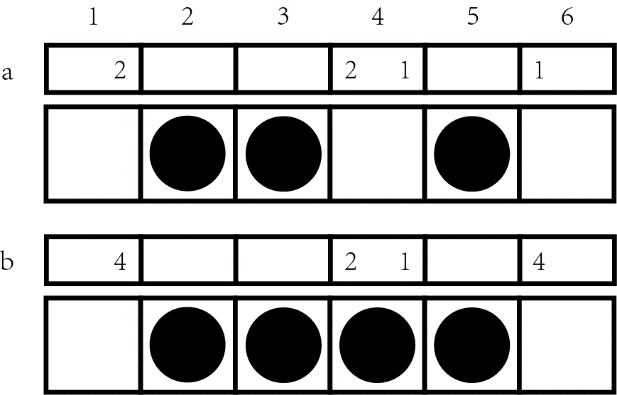
\includegraphics[width=0.5\textwidth]{assets/adjTable.png}
    \caption{邻接信息表示意图}
    \label{fig:adj}
\end{figure}

\paragraph{邻接信息表} 这是我独立发明的一个数据结构,用于加快胜负判断和禁手检查的速度。其作用是保存每一个空的格子周围每个方向上有多少个相邻的相同颜色的棋子。图\ref{fig:adj}所示为此数据结构的简化情况,假设只有黑子,且只有左右两个方向。由a到b的变化展示了在黑子落子后该数据结构中数据的变化情况。在搜索时经常需要回溯,即还原回棋盘上一步的状态。该数据结构中我们可以通过第4格中的数据还原第1和第6格中改变的数据,从而从b还原回a。将此图所示结构扩展到黑白两方(两方分别是独立的),并将左右2个方向扩展到四周8个方向,即是我设计的邻接信息表。

该结构在更新和回退操作时无任何条件判断,实现起来非常方便。该结构在判断胜负时尤为好用,只需检查落子的格子上,有没有两个相对的方向记录的数据之和为4(或更多,视规则而定),若有则落子方胜利。该结构在禁手检查时也有一些作用。

\paragraph{节点缓存} 在节点搜索结束后,并不将搜索结果丢弃,而是动态申请内存将搜索结果保存下来。这样做虽然十分耗费内存,但有以下几个好处:
\begin{itemize}
    \item 当进行更深层的搜索时,再次经过该节点时可以不需要再运行走法生成,而是使用保存的子节点。
    \item 配合转置表使用时,从其他分支搜索到相同的局面时,可能可以重用上次得到的搜索结果
    \item 若下一回合轮到自己走子时再次搜索到这个节点,可能可以重用搜索结果。    
\end{itemize}

\paragraph{模式缓存} 如前文启发评价函数中所述,本引擎使用的启发评价为所有模式评分之和,而每个模式又可分为前后两个部分。当落子(或回溯)时,新的棋子只会影响到其四周8个方向共48个模式部分。新计算的模式部分与缓存中的部分组合成新的完整模式,从而生成新的评分。

\paragraph{走法生成} 为了达到最高的走法生成的速度,我维护了一份所有可行走法的列表,而不是每次都重新生成所有走法。每次落子时都在列表中加入新子周围的8个格子(如果该格子是空的,且没有已经存在于列表中的话),且从列表中删除新子占用的格子(如果该格子在列表中的话)。为了快速检查这些条件,我还维护了一个比特集,以每个bit代表一个格子,记录哪些格子目前在可行走法的列表中。

\paragraph{杀手启发} 每一层记录两个杀手走法,采用简单的FIFO替换策略。

\paragraph{转置表} 从对局生成哈希时使用的算法是Zobrist Hash算法,该算法几乎适用于所有棋类游戏,且其支持基于上一个盘面增量生成哈希值,计算速度较快。转置表的大小会随着条目的增多而自动扩容,但会在每一步完成后清空。

\paragraph{棋盘表示} 在棋盘上下左右各多加一格,并标注为“棋盘外”。这样可以在胜负判断等代码中减少大量边界判断的分支。使用一维数组来保存二维的棋盘,这样可以方便高效地统一各个方向的操作,只需要改变操作的步长即可。例如,向右找下一个格子是找数组的下一个元素,而向下找下一个元素则是找数组的下w个元素,w为棋盘宽度。

\paragraph{对战平台} 为了便于评测引擎的棋力表现受到不同优化手段的影响,我搭建了一个简易的对战平台,允许使用不同参数设置的引擎相互对战。在实现中,由于Alpha Beta搜索算法中没有任何随机性,所以使用相同参数的引擎相互对战多场很可能是完全一样的结果。为了解决这个问题,我在对战平台中引入开局库。即事先为黑白双方下好对双方都较为公平的几步,然后再让双方开始对弈。改变开局即可保证每局比赛不会完全相同。该想法是借鉴piskvork程序的。

\paragraph{单元测试} 实现这些较为复杂的算法设计是比较有挑战性的工作,即使是老师给的示例程序中依然有会导致程序崩溃的bug。为了应对这个问题,我使用了单元测试的方法。目前我编写了42个测试用例,代码测试覆盖率为63\%。单元测试的确帮助我在集成调试之前找出了不少bug。特别是对于复杂的禁手判断规则,在单元测试的帮助下,我对我的禁手判断算法的正确性更有信心了。

\paragraph{性能测试} 对于AI来说,性能是十分重要的,性能越高,搜索的内容就越多,在对弈中就越有优势。为此我专门编写了一个用于性能测试的可执行文件,它直接调用引擎的核心模块。配合第三方的性能评测工具可以很方便的判断代码在哪个部分消耗了更多时间,哪些语句执行的次数更多等等。

\paragraph{模块化} 对于软件来说,可修改性是重要的质量属性。而模块化是实现该质量属性的主要方法。图表 2展示了本程序的模块化层次结构。每一个模块都具有良好的封装,可重用,可替换。

\section{实验}

\paragraph{执行演示} 该引擎的.NET Framework与.NET Core可执行文件均可以正常于piskvork程序中加载运行,并展现出较强的实力。

\paragraph{棋力评测} 本引擎棋力较高,以本人的棋力无法战胜AI。故在评测时只能以其他AI的棋力作为参考。本引擎在班级中举办的比赛中获得了第一的成绩。但是在AI中比较时,老师提供的test程序棋力非常高强,即使本引擎使用10秒搜索时间而test只使用0.5秒,我依然无法战胜它。而且test可以提前20步左右就预见自己的胜利,相比之下本引擎只能提前8步左右。由此看来目前AI所能达到最高的棋力远不止于本引擎的水平。作为棋力的对比,我实现了一个简单的蒙特卡洛树搜索算法,该算法也具有不俗的实力,我本人也无法击败它。

以下评测未经特殊说明均使用2秒/步的时间控制,不带禁手的传统规则,使用指定的开局。为保证公平,同一开局双方各先下一次。

\begin{table}
    \centering
    \begin{tabular}{l l | r @{:} l | c}
        \textbf{引擎1} & \textbf{引擎2} & \multicolumn{2}{c|}{\textbf{比分}} & \textbf{评测方面} \\
        \hline
        本引擎Alpha Beta 10秒/步 & test 0.5秒/步 & 0 & 4\\
        本引擎Alpha Beta & negamax & 30 & 0\\
        本引擎Alpha Beta & 本引擎蒙特卡洛树搜索 & 29 & 1\\
        本引擎蒙特卡洛树搜索 & negamax & 22 & 8\\
        本引擎关闭剪枝 & negamax & 2 & 8 & \ref{item:eff:alphaBeta}\\
        本引擎Alpha Beta & 本引擎关闭杀手启发 & 7 & 3 & \ref{item:eff:killer}\\
        本引擎关闭杀手启发 & 本引擎关闭杀手启发和子节点排序 & 8 & 2 & \ref{item:eff:killer}\\
        本引擎蒙特卡洛树搜索 & 本引擎关闭杀手启发和子节点排序 & 5 & 5 & \ref{item:eff:order}\\
        本引擎Alpha Beta & 本引擎关闭转置表 & 27 & 23 & \ref{item:eff:transpose}\\
    \end{tabular}
    \caption{棋力评测对局记录}
    \label{table:battleRecord}
\end{table}

\subparagraph{评测方面} 表\ref{table:battleRecord}展示了在各个方面的评测记录。
\begin{enumerate}
    \item \label{item:eff:alphaBeta} Alpha Beta剪枝效果:本引擎关闭剪枝和杀手启发后进行评测,以测试Alpha Beta剪枝对棋力做出的贡献。评测时也同时关闭了杀手启发,因为其主要作用是辅助剪枝。
    
    实验结果说明剪枝在棋力的提升中起了重要作用,关闭剪枝后连之前棋力最弱的negamax也敌不过。这可能是因为negamax中的启发评价函数更好的原因。

    \item \label{item:eff:killer} 杀手启发效果:测试杀手启发对棋力的影响。我注意到开启杀手启发的引擎搜索层数一般会多1-2层。
    \item \label{item:eff:order} 子节点排序效果:测试迭代加深中使用浅层搜索结果对子节点进行排序对棋力的影响。测试时将关闭双方的杀手启发,因为杀手启发将代替大多数子节点排序的工作。
    \item \label{item:eff:transpose} 转置表效果:测试转置表对棋力的影响。转置表在棋力的提升中表现并不明显,虽然转置表在第10层时能将搜索的节点数量降低到原来的40\%左右,但转置表本身也会引发一些额外的开销,转置表并未能有效地提高搜索的层数。
\end{enumerate}

\paragraph{棋力评测结果} 图表 4展示了此次棋力评测的结果。test引擎由于棋力太高,未尝败绩,故无法对其棋力做出准确评判,只能说其棋力远高于本次评测中的其他引擎。此处使用Bayesian Elo程序\cite{WEBSITE:BayesianELO}基于以上共计150场对战结果对不同的引擎及其不同配置的棋力进行评分。此处评分结果仅有相对意义,即本表中的分数可以互相比较,但本结果不应与其他地方的Elo评分进行比较。Elo评分的含义如下,其中$e(\cdot)$为玩家的Elo评分。例如当双方分差200分时,强者击败弱者的概率约为76\%。

\begin{equation}
    P(\text{a击败b})=\frac{1}{1+10^{(e(b)-e(a))/400}}
\end{equation}

从图表中我们可以清晰地看到剪枝对棋力的影响是十分巨大的。杀手启发与节点排序对棋力的影响也是较为显著的,而转置表的影响则比较小。简单的蒙特卡洛树搜索算法也拥有不俗的棋力。

\section{未来工作}
\paragraph{启发评价函数} 虽然我不是很愿意,但是Alpha Beta剪枝算法要求要有一个启发评价函数,于是就有了上述启发评价函数。在设计之初,我本希望使用机器学习方法来获得启发评价函数中的权重。但由于时间关系,这项工作并没有进行。目前的构想是,启发评价本质上就是一个二分类器,它输入一个棋局,给出这个棋局赢或者输的概率。而我设计的启发评价函数中的数千个模式的评分便是手动从棋局中提取的特征。机器学习的流程与Alpha Go Zero类似 [3]。先随机初始化模式评分,并让引擎自我对弈,并用对弈中的棋局和对弈的结果作为分类器训练的输入,使用传统的逻辑回归,线性SVM等方法来得到新的评分,再让使用了新的评分的引擎自我对弈,产生新的训练数据,如此循环直至收敛。此模型是线性模型,因此训练的难度和时间要求应该不会太高。此方法虽然减少了人类知识的使用,但是还是使用了五子棋的领域知识来手动提取特征。之所以这样设计,是因为如果使用类似Alpha Go的通用模型,在个人计算机上所需训练时间太长。

\paragraph{其他优化方法} 使用AI进行棋类游戏的研究已经进行了数十年了,在这期间人们发明了不少优化的方法。本文中应用的方法都是比较保守的,即在已搜索完的层数中,保证可以找出所有的杀棋,不会漏搜。但也存在一些更为激进的算法,对于棋力提升应该是很有帮助的。

\paragraph{对照其他实现进行优化} 在实验时老师提供test引擎棋力非常高,但并没有它的源代码。若能参考其实现方法并分析它棋力强的原因,想必是对本引擎棋力提升有帮助的。

\section{总结}

在本次设计、实现与优化的过程中,我体会到即使是运算速度如此快的计算机在搜索时面对巨大的分支因子的无力,体会到剪枝对性能提升的巨大作用。同时我也感受到算法在实现上的困难与权衡,算法实现的效果与想象中的差距。但也从中学习到了设计、构建算法实现,及查错,验证假设的经验。

使用人类知识来设计启发的确能提高AI的实力,但有时却也成为了AI的限制,比如Alpha Go Zero在去除了人类知识后,才获得了超越所有人类,甚至超越了使用了人类知识的自己。而算法的提升却能给AI带来无限的成长空间。本引擎验证了即使简单的启发也可以取得很好的效果,虽然在这里人类知识应该还不至于成为AI的限制。

\bibliography{bibtex} 
\bibliographystyle{ieeetr}

\end{document}
